\documentclass{scrartcl}

\usepackage[latin1]{inputenc}
\usepackage[T1]{fontenc}
\usepackage[ngerman]{babel}
\usepackage{amsmath}
\usepackage{amssymb}
\usepackage{graphicx}

\title{�bung Neuroinformatik - Blatt 09}
\author{Gruppe AC}


\begin{document}
\maketitle

\section*{Aufgabe 1: Gewichtsinitialisierung}
\subsection*{Teilaufgabe 1}

\begin{enumerate}
	\item[a)] \begin{align*}
		F(u_i)  &= \sum_{k=1}^{m} x_k \cdot \mathcal{N} \{ w_{ki}^{(1)} \} \quad ,m=300 \\
				&= \sum_{k=1}^{m/2} 1 \cdot \mathcal{N}(0,1) \\
				&= \mathcal{N} (0, \sqrt{150}) 
	\end{align*}
	
	\item[b)] Die Aufsummierung der Standardnormalverteilungen f�hrt zu der in Abbildung \ref{fig:NV} dargestellten Normalverteilung. Diese ist beinahe gleichverteilt, was mit zunehmendem $m$ verst�rkt wird. Da die Gewichte alle sehr unterschiedlich sind, f�llt der zugeh�rige Gradient ebenfalls sehr unterschiedlich aus. Unter Umst�nden konvergieren manche Gewichte deutlich langsamer als andere. 
	
	\item[c)] \begin{align*}
		F(u_i)  &= \sum_{k=1}^{m} x_k \cdot \mathcal{N} \{ w_{ki}^{(1)} \} \quad ,m=300 \\
				&= \sum_{k=1}^{m/2} 1 \cdot \mathcal{N}(0, 1/\sqrt{m} \\
				&= \mathcal{N} \left(0, \sum_{k=1}^{m/2} \left( \frac{1}{\sqrt{m}}\right)^2 \right) = \mathcal{N} \left(0, \sum_{k=1}^{m/2} \frac{1}{m} \right)\\
				&= \mathcal{N} \left(0, 0.5 \right)
	\end{align*}				
			
	\item[d)] Die Aufsummierung der \emph{truncated normal distribution} f�hrt nicht zu einem so gro�en Sigma-Wert der resultierenden Verteilung. (vgl. Abbildung \ref{fig:tnd}	
\end{enumerate}

\begin{figure}
	\centering
	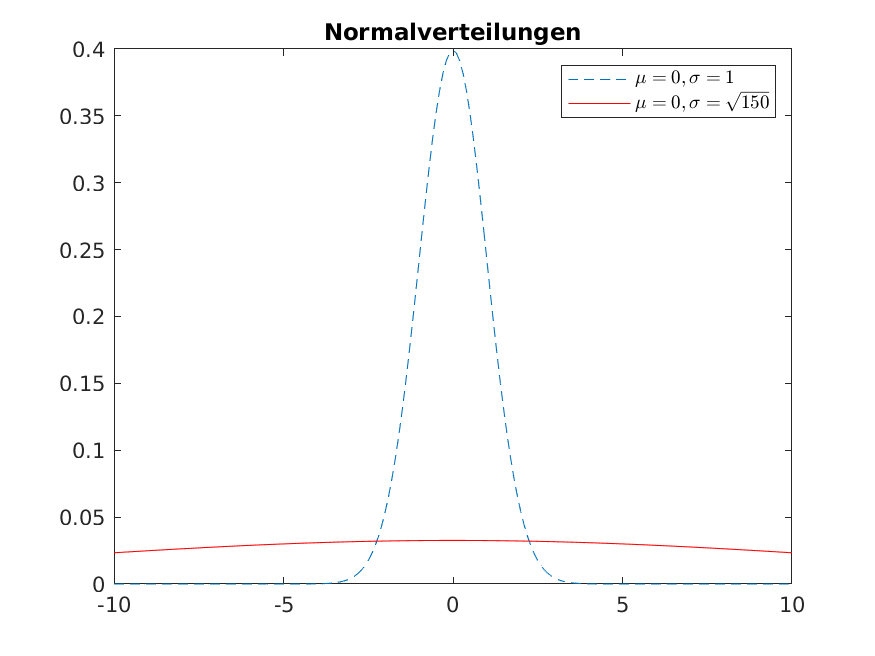
\includegraphics[width=0.8\linewidth]{verteilung} 
	\caption{Normalverteilungen zu Teilaufgabe 1b}
	\label{fig:NV}
\end{figure}

\begin{figure}
	\centering
	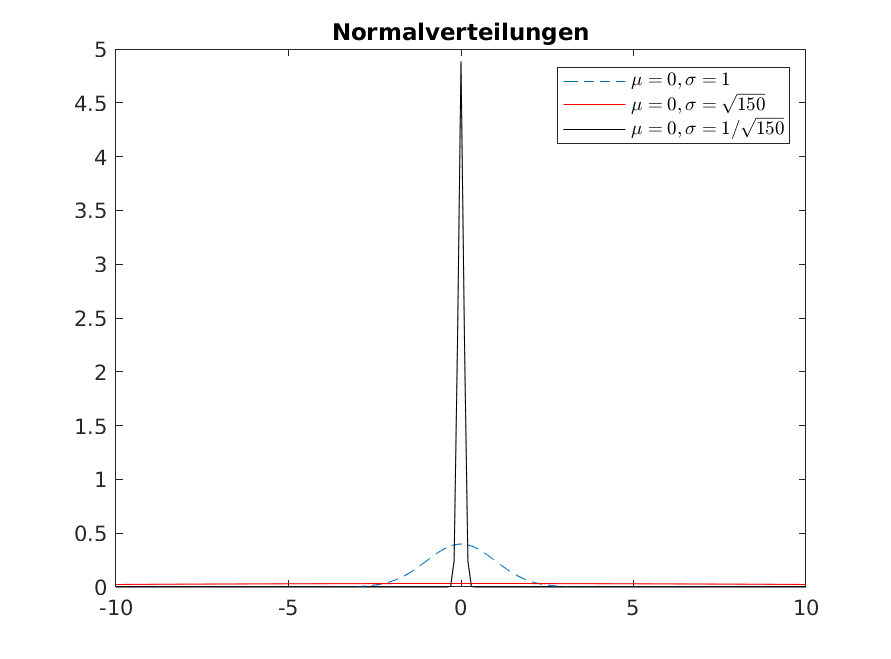
\includegraphics[width=0.8\linewidth]{tnd} 
	\caption{Normalverteilungen zu Teilaufgabe 1d}
	\label{fig:tbd}
\end{figure}

\section*{Teilaufgabe 2}
\begin{enumerate}
	\item[A] entspricht der skalierten Normalverteilung: Die Gewichte sind entsprechend der in Teilaufgabe 1 berechnete Normalverteilung verteilt. 
	\item[B] entspricht der Standardnormalverteilung: Die Gewichte und axonalen Potentiale sind nahezu gleichverteilt. (Vgl. Teilaufgabe 1b)
\end{enumerate}

\section*{Teilaufgabe 3}
\begin{enumerate}
	\item[Problem] In der gegebenen Formel zur Berechnung des Gradienten kommt der Term $\sum_{i=1}^{n}w_{ij}^{(2)}\cdot x_k$ vor. Da $w_{ij}^{(2)}$ wie in Teilaufgabe 1 auch Normalverteilt ist, tritt hier der gleiche Effekt/ das gleiche Problem auf. Durch Aufsummierung addieren sich die Standardabweichungen zu einem gro�en Wert auf. Die Gradienten sind dann sehr unterschiedlich gro�.
	\item[L�sung] Durch die Xavier-Initialisierung wird analog zur Teilaufgabe 1c) die Verteilung derma�en geschm�lert, dass die Summe der Verteilungen wiederum akzeptable Kennwerte aufweist.
\end{enumerate}
\end{document}